\chapter{插件详细设计与实现}

\section{单元测试插件}

本插件与本软件内核高度耦合,随内核更新而更新。本插件仅用于开发者进行测试,对普通用户没有意义。

本插件能够以多种方式构造多个测试用例,测试内核和默认附加插件的正确性、鲁棒性和安全性。同时,它可以测试插件的可用性。

\section{文件信息统计插件}

本插件能够从全局角度下统计文件信息,以文件类型、文件标签等方式,以图表的形式展示出来。

\begin{figure}[h]
    \centering
    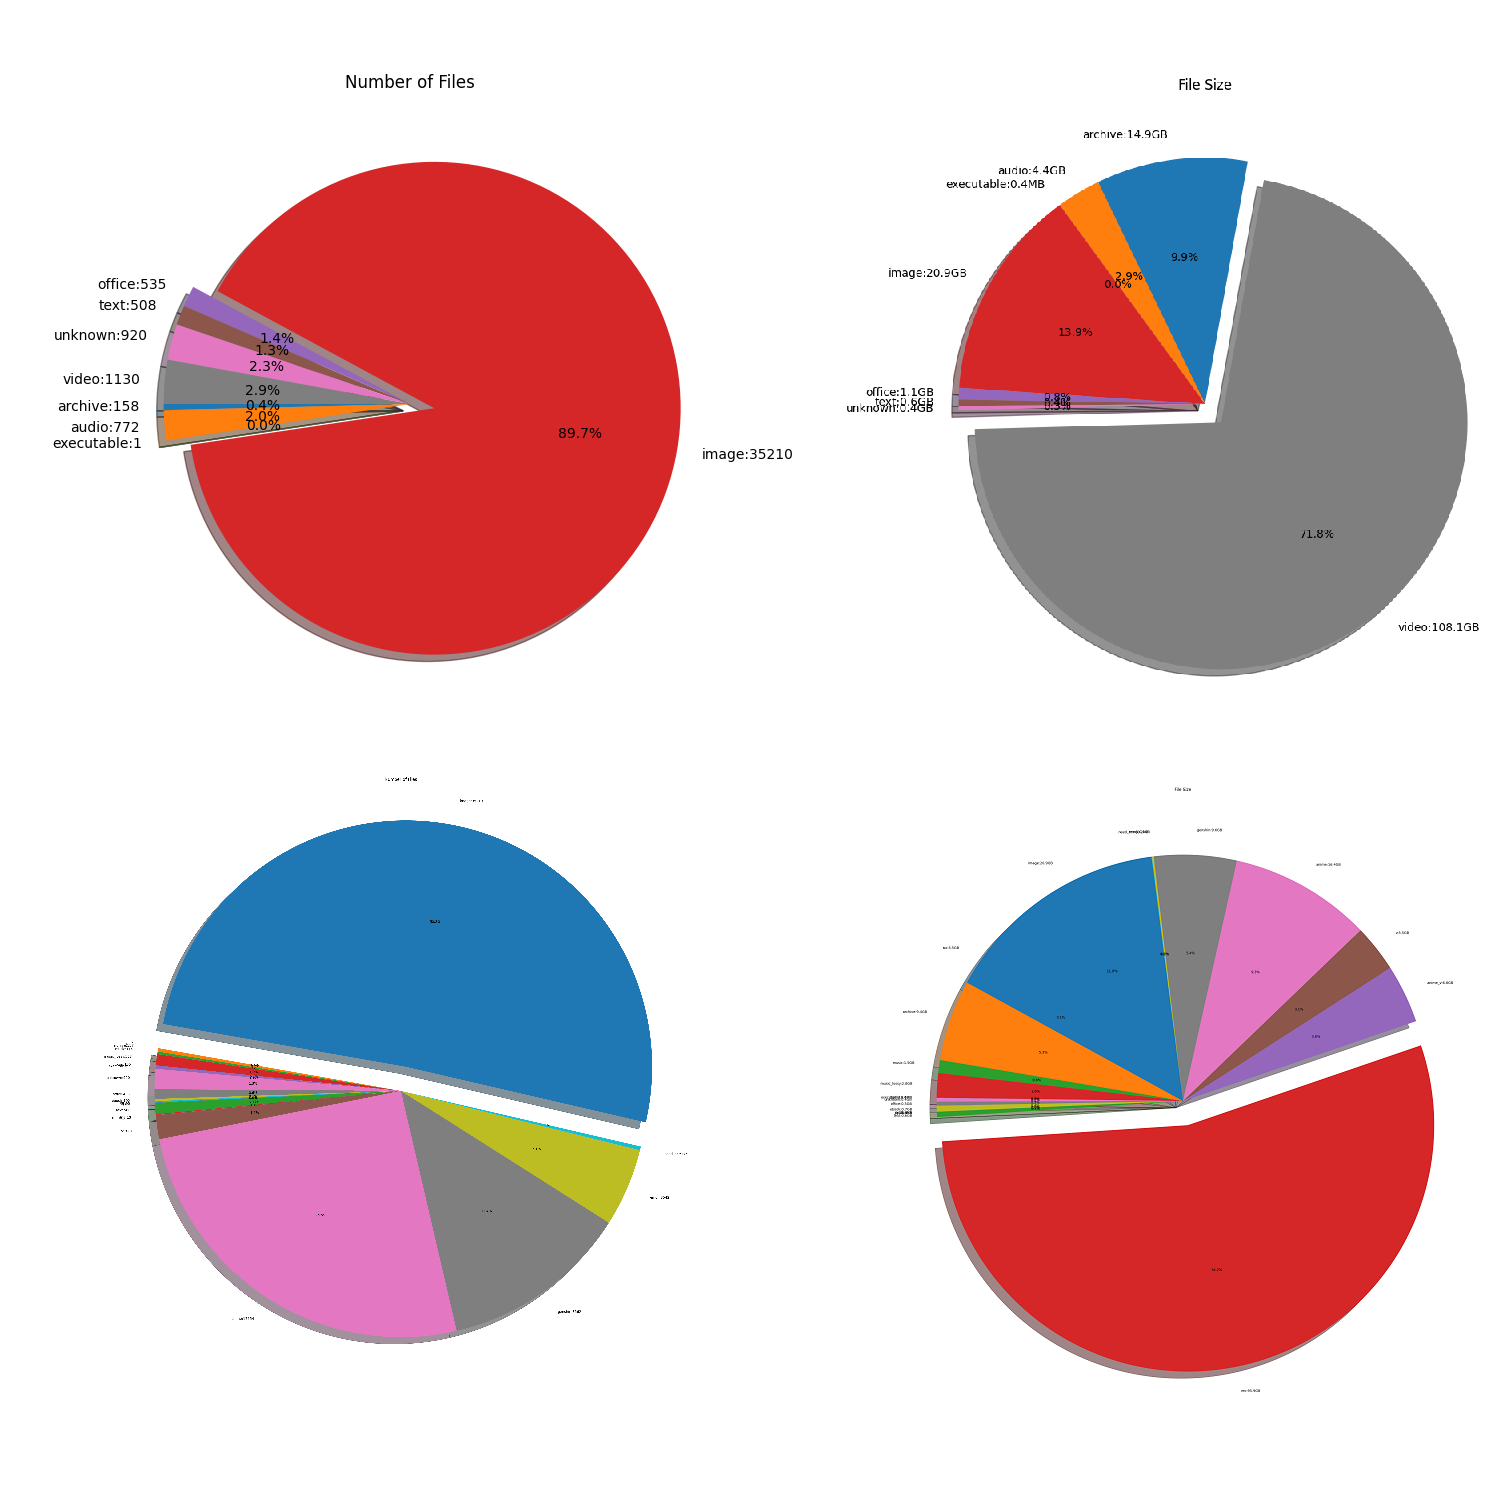
\includegraphics[width=\textwidth]{figures/pie4.png}
    \caption{文件统计信息}
    \label{fig:pie4}
\end{figure}

如图 \ref{fig:pie4} 所示,本插件分别以文件类型、文件标签的方式,展示了文件统计信息的饼形图。其中,由于存在一个文件有多个标签的情况,所以文件标签相关的图表中数据之和大于总数。

\section{基于 ANSI 控制符的文件信息查看插件}

本插件为命令行界面(Command-Line Interface, CLI)插件,能够以用户友好的方式显示文件信息。

本插件基于 ANSI 控制符实现界面刷新、文本位置控制、文本高亮等特性。

\section{基于多用途互联网邮件扩展的归类整理插件}

本插件继承了插件管理系统的插件类 \tt{PluginDestination} 类,通过文件多用途互联网邮件扩展的类型将文件归类并整理。本插件(类)的目标地址检查方法为依次检查根文件夹和子文件夹的存在性以及是否为文件夹。

本插件依赖于基于多用途互联网邮件扩展的标签生成插件。

\section{基于 FFmpeg 的媒体文件信息分析插件}

本插件继承了插件管理系统的插件类 \tt{PluginAnalysis} 类,通过命令行调用 FFmpeg 中的命令行工具 ffprobe 分析媒体文件,并将信息记录在信息类 \tt{Info} 中。

\section{基于散列的相同文件检索插件}

本插件计算文件的 SHA256 并记录到数据库,通过比较文件的 SHA256 是否相同来判断是否是同一个文件。

基于 SHA256 算法的雪崩效应,文件的 SHA256 的分布是随机、均匀的。因此,可以通过分块算法优化时间复杂度:将文件的 SHA256 的前 16 位作为“桶”的键,将文件记录到对应的桶内,检索相同文件时只在桶内检索。分块算法可将比较逻辑的时间复杂度从 $O(n^2)$ 优化到 $O(n^2/m^2)$,其中 $n$ 为文件数量,$m$ 为桶的数量。

\section{基于感知散列的相似图像检索插件及其优化}

本插件计算文件的 64 位感知散列值并记录到数据库,通过感知散列值的汉明距离来衡量两个文件的相似度。

检索相似图像有两种检索方式:非传递性检索和传递性检索。

\subsection{非传递性检索}

非传递性检索指检索时仅检索与目标图像感知散列值的汉明距离小于某个值的图像。非传递性检索 Python 代码如下:

\begin{lstlisting}[language=Python]
def intransitive_search(img_phash: int, distance: int) -> list:
    return [i for i in data if hamming_distance(data[i], x) < d]
\end{lstlisting}

\subsection{传递性检索}

传递性检索指检索时将与目标图像(集合)感知散列值的汉明距离小于某个值的图像加入目标图像集合,重复递归检索,直到检索不到相似图像。

并查集(Disjoint-set data structure)是一种数据结构,用于处理不交集(Disjoint sets)的合并及查询问题。在传递性检索前,可以通过并查集预处理数据,以优化时间复杂度。并查集最优、最常见的实现为记忆化(memoization,是一种典型的在计算时间与电脑存储器空间之中获取平衡的方案)优化不交集森林(Disjoint-set forest)。此算法空间复杂度为 $O(n)$,每次查询的时间复杂度从 $O(n)$ 优化到 $O(\alpha(n))$,其中 $n$ 为图像数量,$\alpha$ 为反阿克曼函数 \cite{dsf}。反阿克曼函数 $\alpha^{-1}(n) = A(n, n)$,其中 $A$ 为阿克曼函数。由于阿克曼函数的增加速率非常快,因此其反函数 $\alpha$ 则会以非常慢的速度增加,考虑到现代文件系统的限制,本软件涉及到的 $\alpha(n)$ 取值均小于 $4$ \cite{a_1} \cite{a_2} \cite{a_3}。

对于每个可能的汉明距离,需要一个不交集森林数据结构。依次创建不交集森林类并初始化,搜素方法为 \tt{find}。令 \tt{data} 为以汉明距离为键,以汉明距离对应的不交集森林类为值的字典,传递性检索 Python 代码如下:

\begin{lstlisting}[language=Python]
def transitive_search(img_phash: int, distance: int) -> list:
    root = data[distance].find(img_phash)
    return [i for i in range(n) if data[distance].find(i) == root]
\end{lstlisting}

\subsection{分块优化}

本插件同样可以通过分块算法进行优化。令 $L$ 是感知散列值 $p$ 位数,即 $L = \rm{len}(p)$。通常,$L = 64$。对于给定的相似度阈值 $d$,令分块数量 $m = \max(L/16, d+1)$。对于每个图像,将其感知散列值 $p$ 分为 $m$ 个感知散列块: $p_i, i \in \bb{N} \cap [1, m]$,每块的大小为 $\lceil L/m \rceil$ 或 $\lfloor L/m \rfloor$,且保证

\begin{equation}
\sum_{i=1}^m {\rm len} (p_i) = L.
\end{equation}

对于每个图像,根据每个感知散列块生成索引字典:字典的键为感知散列块 $p_i$ 及其序号 $i$,值为一个图像序列。

分块数量 $m = \max(L/16, d+1)$ 可以保证 $m \geq L/16$ 且 $m > d$。当 $m > d$ 时,必然存在某个感知散列块 $p_i$,使得相似(即汉明距离小于等于 $d$)的图像图片对被存放到 $p_i$ 中的同一个索引 \cite{phash3}。因此,所有相似的图片对都必然能被本算法检测到,保证了本算法的正确性。

分块数量 $m \geq L/16$ 可以保证

\begin{equation}
{\rm len} (p_i) \leq 16, \forall i \in \bb{N} \cap [1, m],
\end{equation}

感知散列块大小不超过 $16$ 位,这使得索引大小不超过 $L/16*2^{16}$,防止了内存的溢出。

本优化方式可同时应用于非传递性检索和传递性检索两种检索方式 \cite{phash3}。

\section{基于 PyParsing 的递归下降集合运算解释器插件}

本插件不依赖于内核,可独立导入(import)、初始化和运行,完成特定的功能。

\subsection{文法设计}

文法 $G$ 定义为四元组 $G=(V_T, V_N, S, P)$,其中 $V_T$ 是有限的终极符集合,$V_N$ 是有限的非终极符集合,$S$ 是开始符且 $S \in V_N$,$P$ 是产生式的集合。

定义文法 $G_0$:

\begin{equation}
\begin{aligned}
G_0 &= (V_T, V_N, S, P),\\
V_T &= \{w\sim()+\},\\
V_N &= \{E\},\\
S &= E,\\
P &= \{E \to w | (E) | \sim E | E+E\},
\end{aligned}
\end{equation}

其中,终极符 $w$ 是匹配正则表达式 \tt{\^{}\textbackslash w+\$} 的字符串,实际意义是一个文件标签的名称;终极符 $+$ 是匹配正则表达式 \tt{\^{}(\textbackslash||\&)\$} 的字符串,实际意义是一个集合运算(\tt{|} 为集合的并,\tt{\&} 为集合的交);其它终极符 $\sim$、$($ 和 $)$ 均是等于其自身字符的字符串。

定义本插件讨论的集合运算表达式的全集 $A$,则一个集合可以表示为一个 $|A|$ 位的二进制数,每一位的取值为某个元素是否存在于此集合中。此时,集合的交、并、取反与布尔值的与、或、非相对应,集合进行运算的结果表示的二进制数,与集合表示的二进制数进行对应运算的结果相同。从布尔表达式的角度来讲,本插件满足的运算满足功能完备性。

\subsection{文法等价变换}

短语文法具有形式 $\alpha \to \beta, \beta \in (V_T \cup V_N)*$,并且 $\alpha$ 至少含一个非终极符;上下文相关文法是短语文法的特例,要求 $|\alpha| \leq |\beta|$,$S \to \alpha$ 例外,但是 $S$ 不得出现于产生式右部;上下文无关文法是上下文相关文法的特例,要求产生式左部是一个非终极符 $A \to \beta$ \cite{compilers}。

文法 $G_0$ 是 0 型文法,但不是 1 型文法。考虑对文法 $G_0$ 进行等价变换。通过增加拓广产生式,消除空产生式,消除左递归等方法,得到文法 $G$:

\begin{equation}
\begin{aligned}
G &= (V_T, V_N, S, P),\\
V_T &= \{w\sim()+\},\\
V_N &= \{EE'TF\},\\
S &= E,\\
P &= \{\\
    &\quad\begin{aligned}
        E &\to TE',\\
        E' &\to +TE' | \varepsilon,\\
        T &\to \sim T | F,\\
        F &\to w | (E)\\
    \end{aligned}\\
&\}.
\end{aligned}
\end{equation}

文法 $G$ 是上下文无关文法。

\subsection{文法分析}

求得各非终极符的 $\rm First$ 集和 $\rm Follow$ 集:

\begin{equation}
\begin{array}{llcll}
{\rm First}(F)  &= \{ w ( \}, & \quad &
{\rm Follow}(F) &= \{ + ) \# \}, \\
{\rm First}(T)  &= \{ \sim w ( \}, & \quad &
{\rm Follow}(T) &= \{ + ) \# \}, \\
{\rm First}(E') &= \{ + \varepsilon \}, & \quad &
{\rm Follow}(E')&= \{ ) \# \}, \\
{\rm First}(E)  &= \{ \sim w ( \}, & \quad &
{\rm Follow}(E) &= \{ ) \# \}.
\end{array}
\end{equation}

求得各产生式的 $\rm Predict$ 集:

\begin{equation}
\begin{array}{lll}
{\rm Predict}(E \to TE'         ) &= {\rm First} (TE'   ) &= \{ \sim w ( \},\\
{\rm Predict}(E'\to +TE'        ) &= {\rm First} (+TE'  ) &= \{ + \},\\
{\rm Predict}(E'\to \varepsilon ) &= {\rm Follow}(E'    ) &= \{ ) \# \},\\
{\rm Predict}(T \to ~T          ) &= {\rm First} (~T    ) &= \{ \sim \},\\
{\rm Predict}(T \to F           ) &= {\rm First} (F     ) &= \{ w ( \},\\
{\rm Predict}(F \to w           ) &= {\rm First} (w     ) &= \{ w \},\\
{\rm Predict}(F \to (E)         ) &= {\rm First} ((E)   ) &= \{ ( \}.
\end{array}
\end{equation}

\subsection{递归下降实现}

基于上述分析,结合 Python 模块 PyParsing,将集合运算表达式字符串转化为一个多层嵌套的表达式队列类(本文称此类为 \tt{ppList})的对象:队列的元素为终极符或 \tt{ppList} 对象。此过程独立于本软件内核。

若需要进一步解析,则需要提供给 \tt{ppList} 对象查询数据库的方法,此方法应返回一个集合,如返回“有某标签的文件集合”的方法。此插件将根据返回的集合,递归地利用符号栈和数据栈对 \tt{ppList} 对象进行解析运算,并最终返回一个集合。此过程 Python 伪代码如下:

\begin{lstlisting}[language=Python]
def interpreter(l: ppList) -> set:
    stack = new_stack()
    for i in l:
        if isinstance(i, ppList):
            i = interpreter(l)
        stack.append(i)
        if stack.is_calculatable():
            stack.calculate()
    return stack.get_result()
\end{lstlisting}

\section{基于集合运算解释器的检索插件}

本插件能通过给出的简单或复杂集合运算语句检索满足相应标签要求的图片。

本插件依赖于基于 PyParsing 的递归下降集合运算解释器插件,通过提供给 \tt{ppList} 对象查询数据库的方法,完成从集合运算表达式字符串到集合的过程。此过程保证确定性。

\section{基于文件标签的归类整理插件}

本插件继承了插件管理系统的插件类 \tt{PluginDestination} 类,通过文件元信息和标签将文件归类并整理。本插件(类)初始化时及实例化后可以添加多条文件元信息和标签匹配规则,规则默认支持子串、子序列、正则表达式,可选支持集合运算表达式。若需要支持集合运算表达式,则需要引入基于 PyParsing 的递归下降集合运算解释器插件,通过提供给 \tt{ppList} 对象查询数据库的方法,完成从集合运算表达式字符串到集合的过程。

当注册事件发生时,本插件根据给定的优先级依次匹配规则,直到匹配到文件对应的最优目标地址为止。此匹配过程保证确定性。

本插件(类)的目标地址检查方法为依次检查每个可能作为目标地址文件夹的文件夹的存在性以及是否为文件夹。

本插件是基于多用途互联网邮件扩展的归类整理插件的增强。

\section{基于 Flask 的 GUI 插件}

本插件基于前端渲染架构,通过 flex css 实现了响应式布局的图片浏览网页。本网页保证图片的长宽比例不变,每行图片行的高相同,且保证图片的顺序。容易证明,在这种情况下,左右的留白是不可避免的。为保证展示效果,采用左对齐的策略。图片默认为圆角,但当鼠标移动到图片上时,图片将在原位置以 1.2 倍放大并产生阴影,同时四角变为直角。

对于图像文件,直接以 \tt{img} 元素插入网页中;对于其它文件,使用 Python 生成临时预览图,再将预览图以 \tt{img} 元素插入网页中。对于每个 \tt{img} 元素,都用一个 \tt{a} 元素包裹,然后修改 \tt{a} 元素的 \tt{href} 属性,以达到点击图片(预览图)访问原文件的功能。

网页渲染完成后,通过 Python 模块 flask 实现网页和程序的通信。

本插件可以连接基于散列的相同文件检索插件、基于感知散列的相似图像检索插件、基于分块加速和感知散列的相似图像快速检索插件、基于集合运算解释器的检索插件和基于文件标签的归类整理插件,通过插件返回文件地址列表的方法进行展示。

\begin{figure}[h]
    \centering
    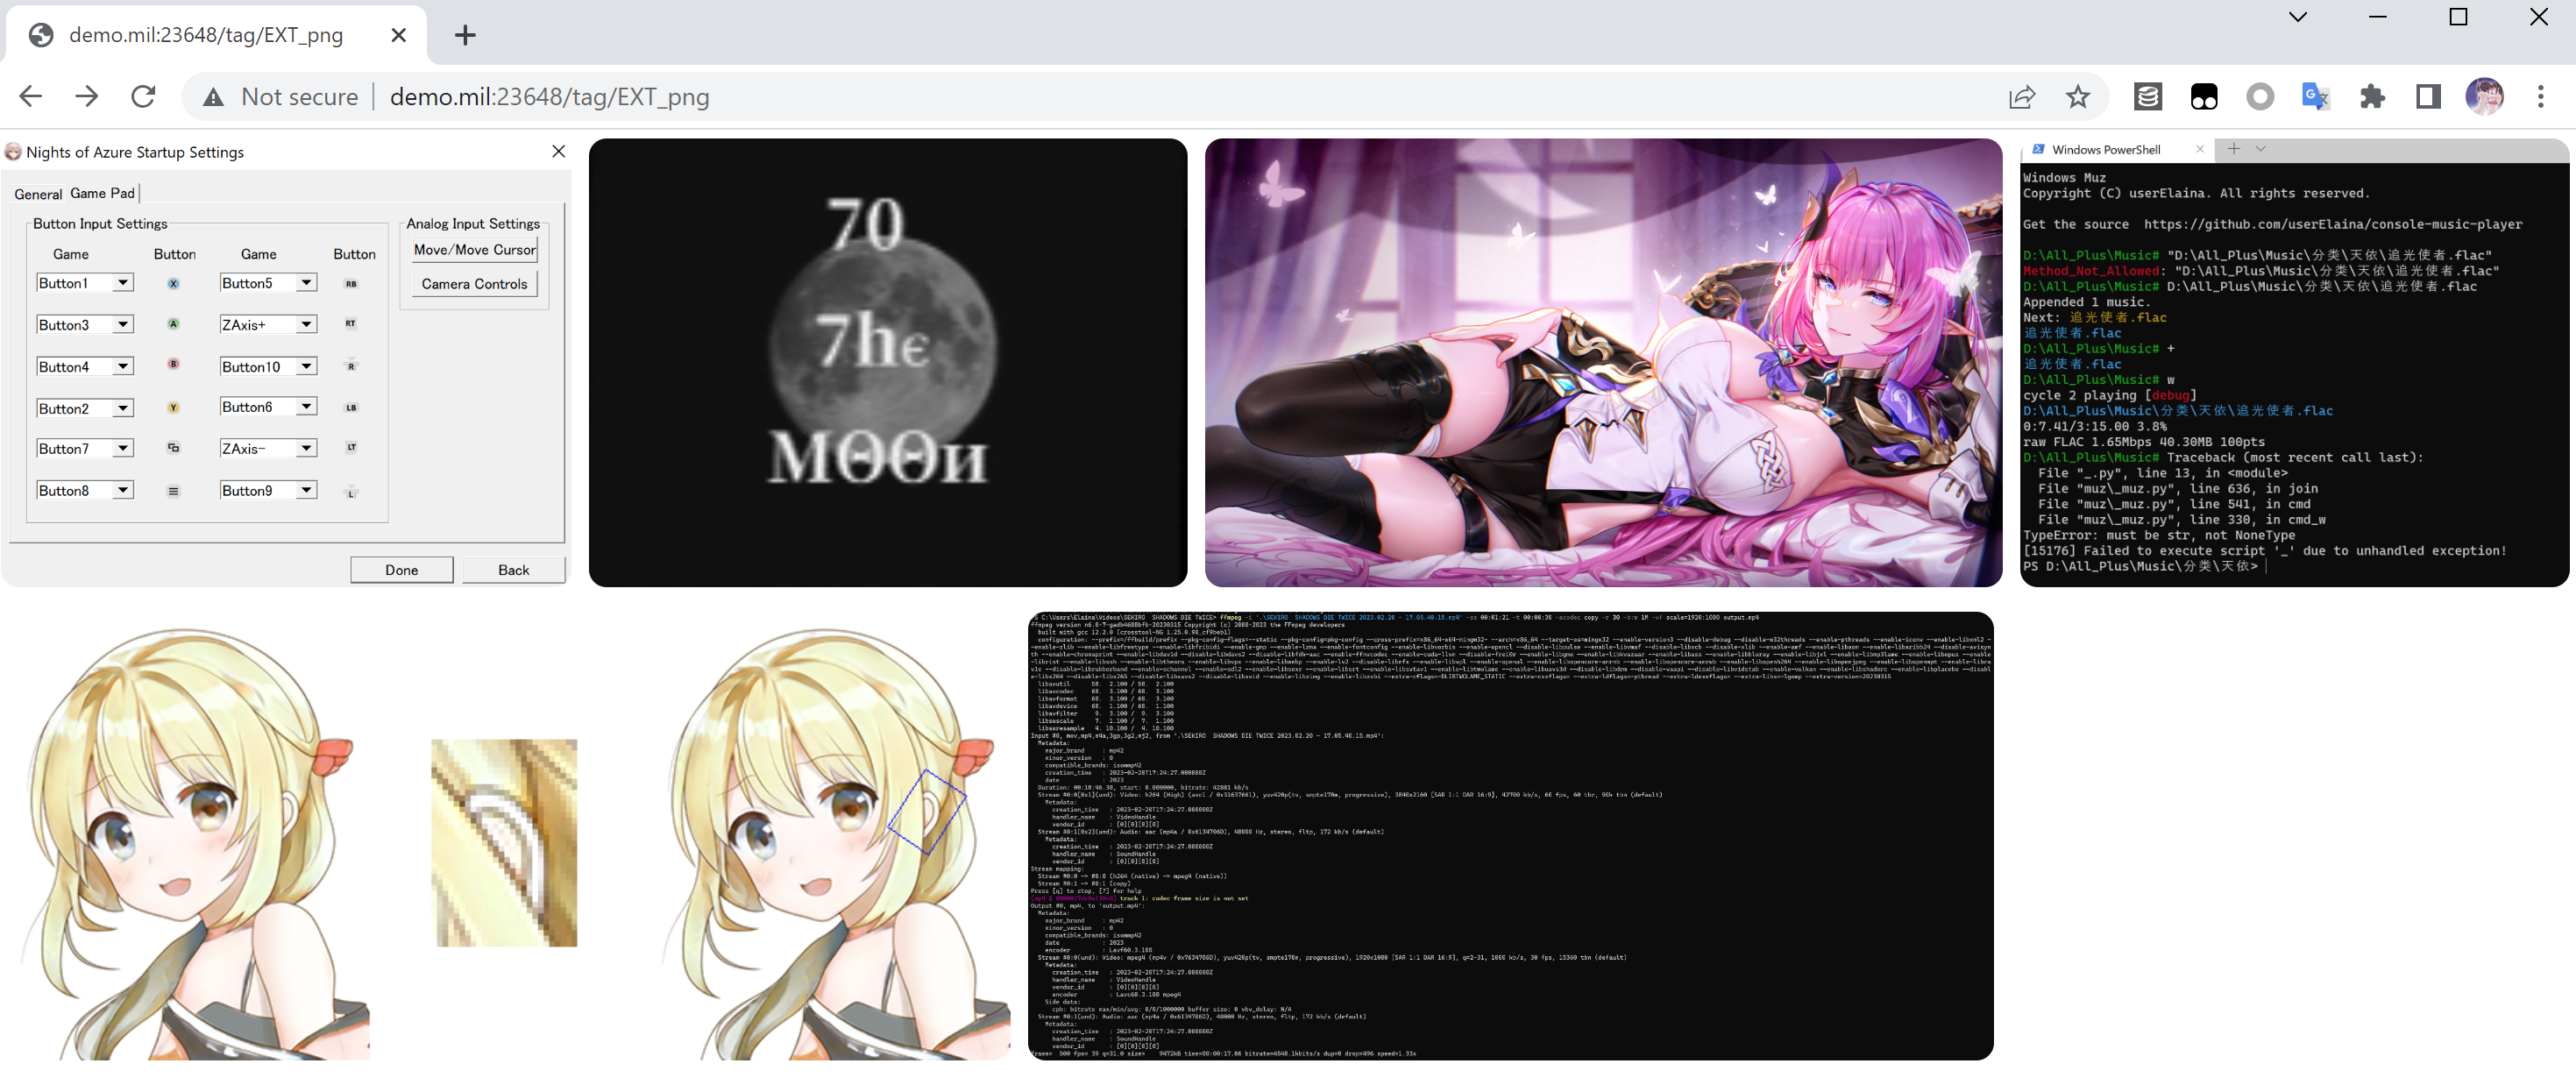
\includegraphics[width=\textwidth]{figures/flask1.png}
    \caption{网页展示:简单表达式}
    \label{fig:flask1}
\end{figure}

如图 \ref{fig:flask1} 所示,\tt{tag/} 后参数为一个简单的集合运算表达式 \tt{EXT\_png}(一个标签)。该网页显示了所有具有标签 \tt{EXT\_png} 即后缀为 \tt{png} 的文件。

\begin{figure}[h]
    \centering
    
\includegraphics[width=\textwidth]{figures/flask2.png}
    \caption{网页展示:复杂表达式}
    \label{fig:flask2}
\end{figure}

如图 \ref{fig:flask2} 所示,\tt{tag/} 后参数为一个复杂的集合运算表达式。该网页显示了所有符合该表达式的文件。其中,后缀为 \tt{py} 的文件为文本文件(Python 代码文件)。文本文件不是图像,不能直接显示,因此,本插件使用 Python 模块 Pillow 将文本绘制在图片上,保存为临时文件,然后显示。

\begin{figure}[h]
    \centering
    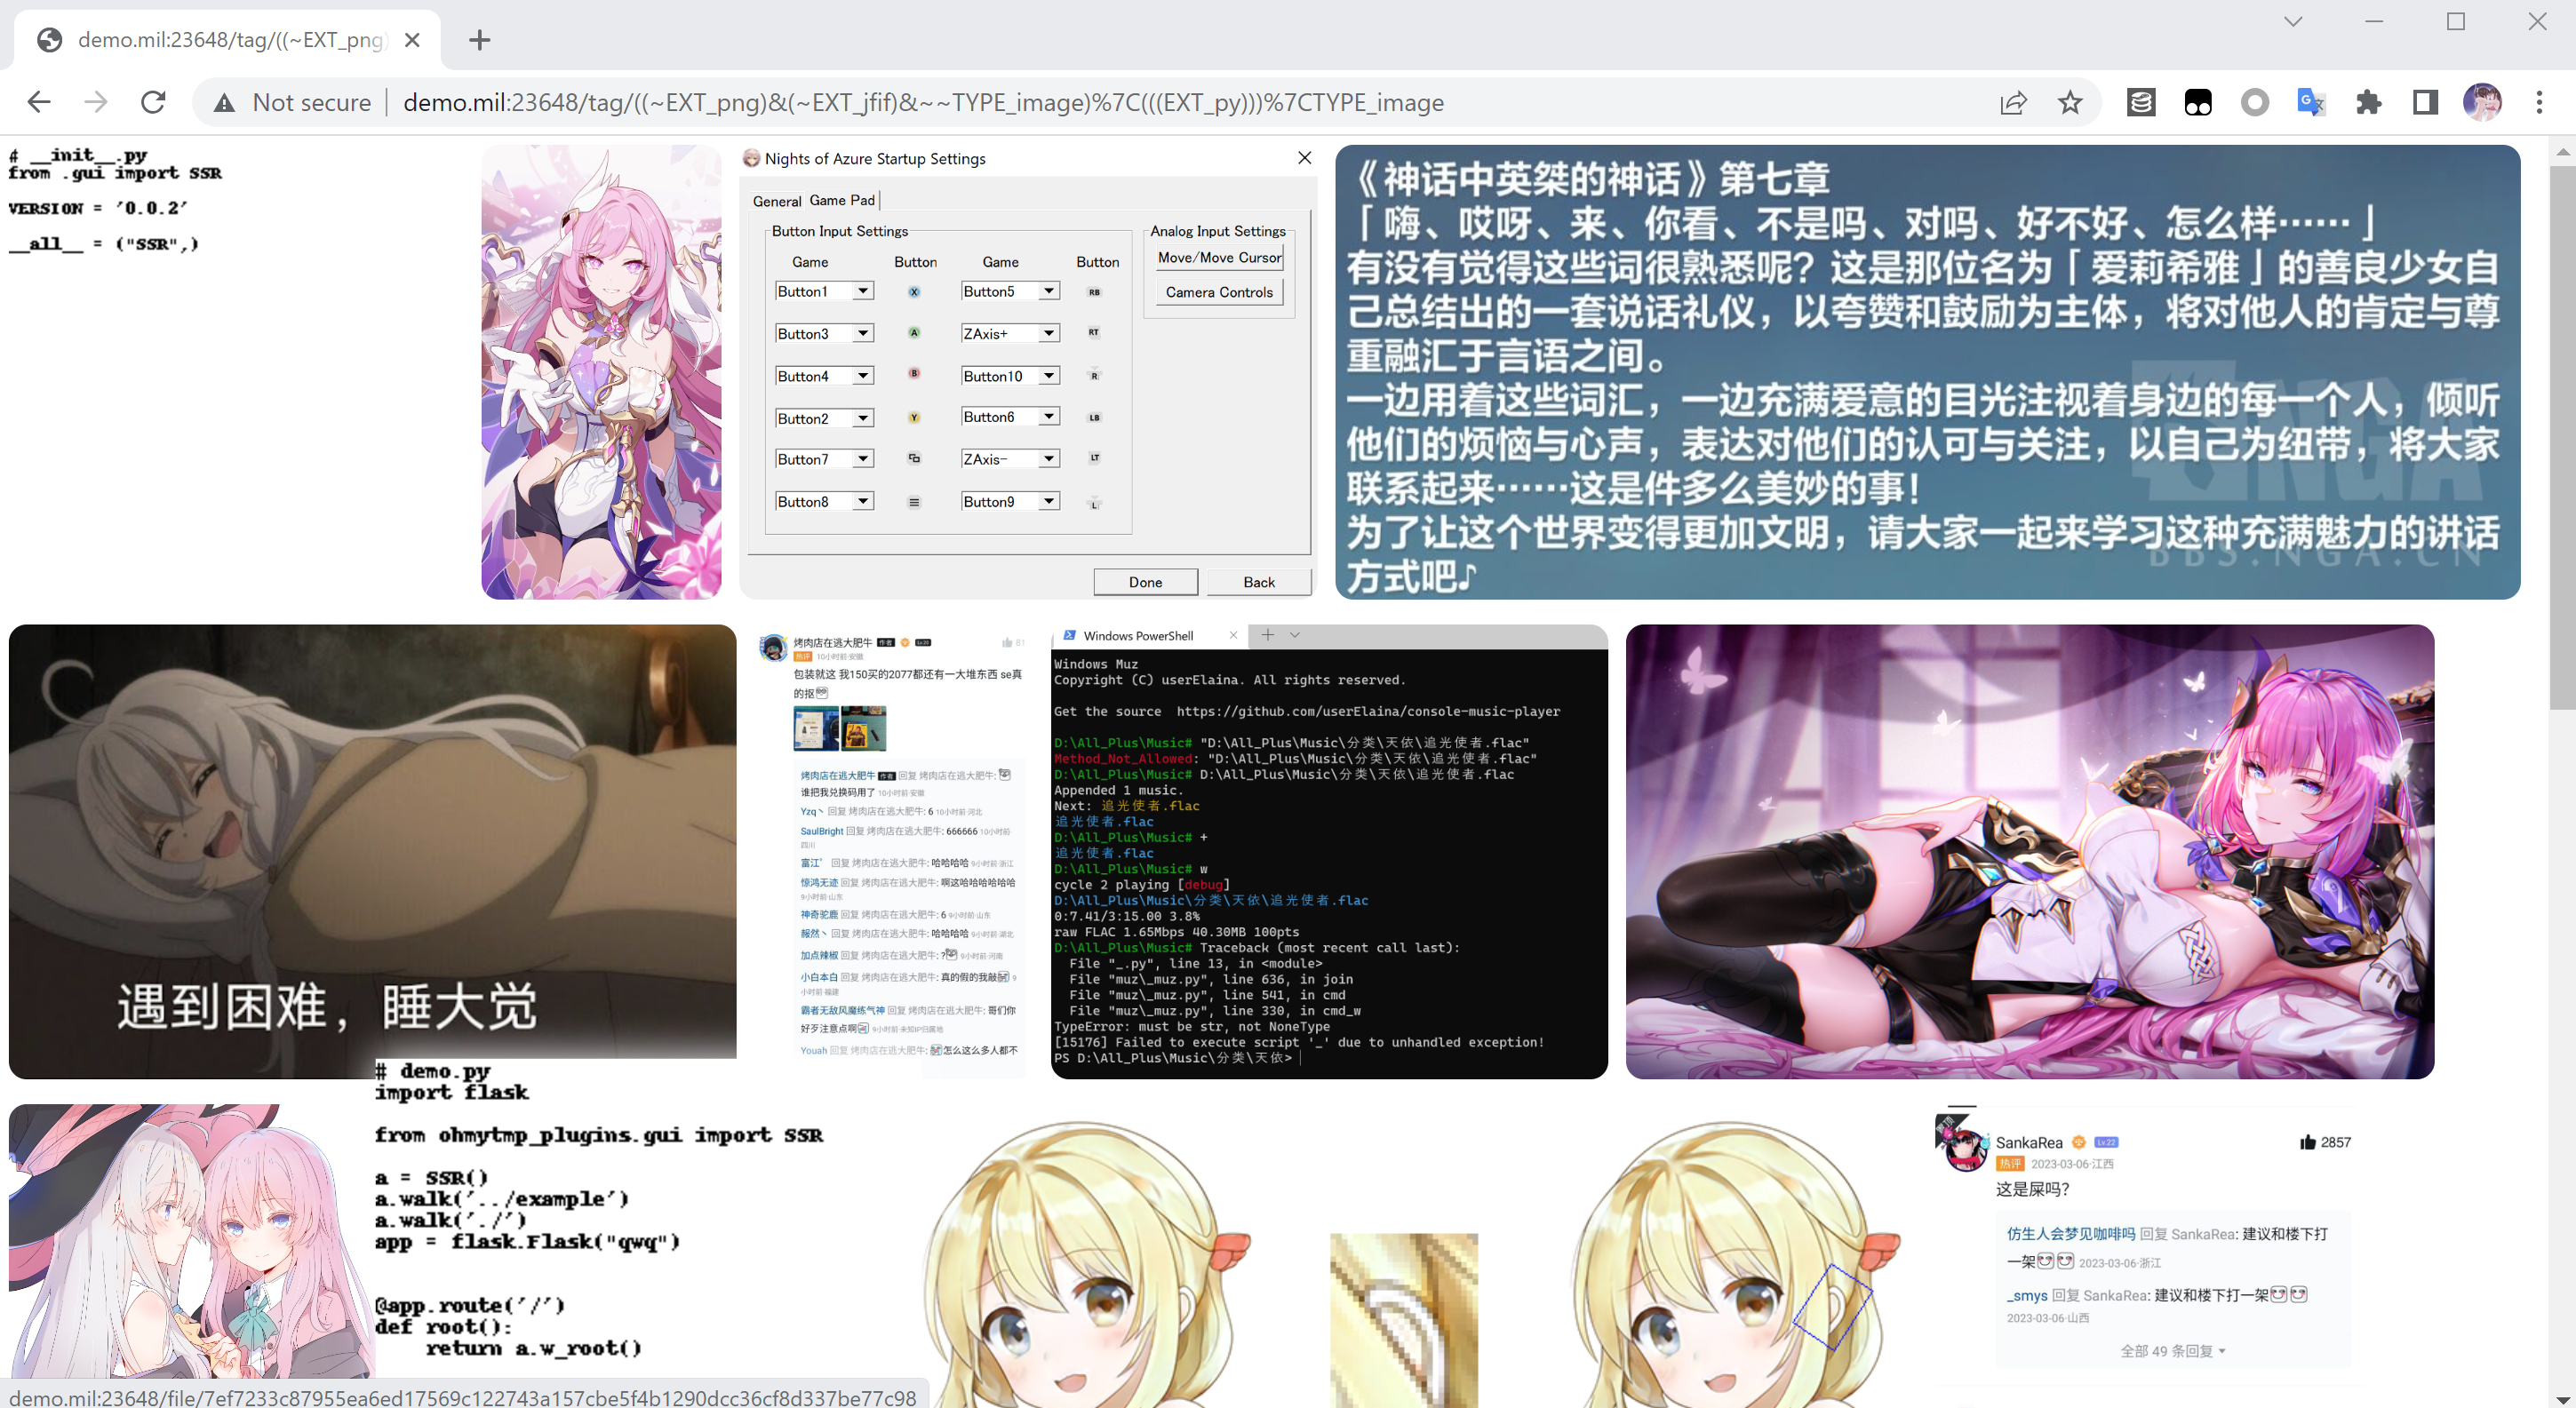
\includegraphics[width=\textwidth]{figures/flask3.png}
    \caption{网页展示:正确性验证}
    \label{fig:flask3}
\end{figure}

如图 \ref{fig:flask3} 所示,\tt{tag/} 后参数为一个简单的集合运算表达式 \tt{TYPE\_image}(一个标签)。该网页显示了所有具有标签 \tt{TYPE\_image} 即(通过其它插件预测的)文件类型为 \tt{image} 的文件。其包括后缀为 \tt{png} 的文件,不包括文本文件。将图 \ref{fig:flask3} 与图 \ref{fig:flask1} 和图 \ref{fig:flask2} 比较,可以在一定程度上验证集合运算表达式解释器的正确性。

\section{基于粒子群优化的子图匹配插件}

相对于暴力搜索算法,粒子群优化虽然无法保证找到的局部最优解是理论最优解,但是其时间复杂度比暴力搜索算法低很多个数量级 \cite{psoimg2} \cite{psoimg3}。

\begin{figure}[h]
    \centering
    
\includegraphics[width=\textwidth]{figures/pso.png}
    \caption{基于粒子群优化的子图匹配}
    \label{fig:pso}
\end{figure}

如图 \ref{fig:pso},本插件通过粒子群优化,能够在原图中匹配裁剪、旋转、缩放后的子图 \cite{git_pso}。此过程独立于本软件内核。

对粒子群优化而言,待优化变量为缩放的倍率和旋转的角度。若损失函数选择平均平方误差(mean-square error, MSE),则可以通过前缀和优化和记忆化,将计算损失函数的时间复杂度从 $O(n^2)$ 优化到 $O(1)$。

\section{基于 GoogLeNet 的图像标签生成插件}

本插件继承了插件管理系统的插件类 \tt{PluginAddTags} 类,通过 GoogLeNet 预训练得到的模型给预测图像文件的标签。在使用 GoogLeNet 执行迁移转移学习时,最常见的方法是使用在 ImageNet 数据集上预训练的网络 \cite{ggnet2}。本插件采用的就是这种方法。

\begin{figure}[h]
    \centering
    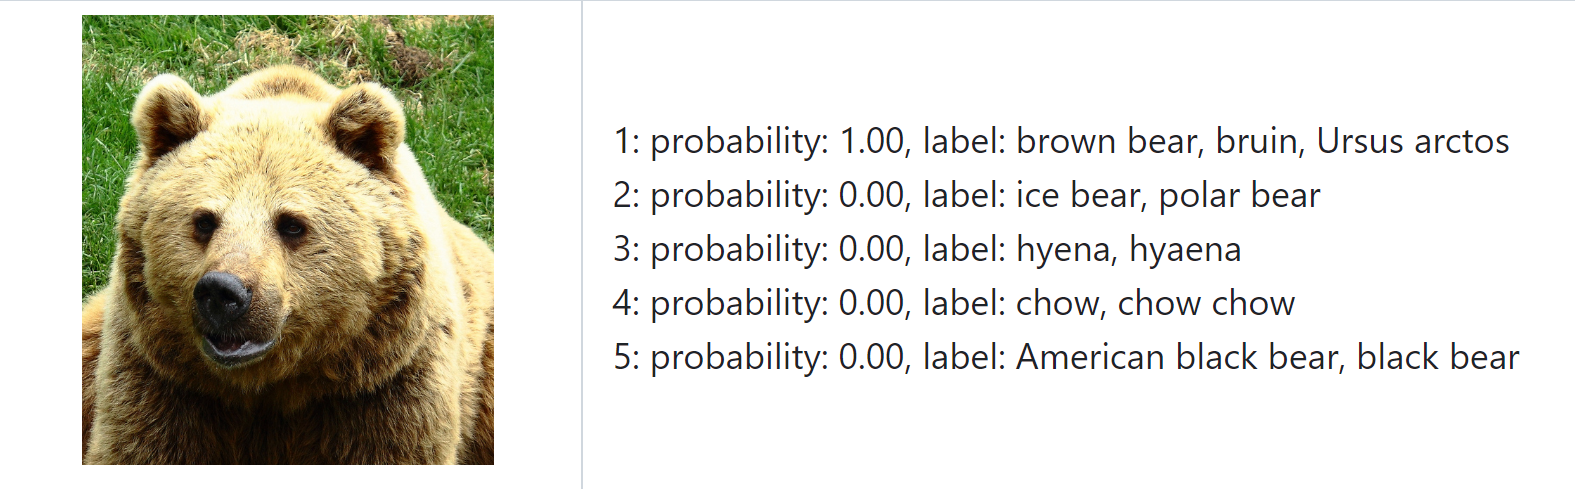
\includegraphics[width=\textwidth]{figures/ggnet.png}
    \caption{GoogLeNet 一次预测的结果}
    \label{fig:ggnet}
\end{figure}

本插件修改自开源项目 GoogLeNet-Inception。此项目基于深度学习框架 TensorFlow 对 GoogLeNet 进行了 Python 实现,但是仅适配少量版本 TensorFlow (要求 TensorFlow 版本不低于 1.9,且低于 2.0)\cite{git_ggnet}。本插件对其进行了修改,使其适配 2.0 及以上版本的 TensorFlow。

若将本软件内核仅和本插件结合考虑,主要的性能开销和代码实现工作,均集中于本插件部分。本软件可以作为机器学习训练的辅助软件进行使用和二次开发,体现了本软件的高可拓展性。
